\begin{figure}[h]
    \centering
    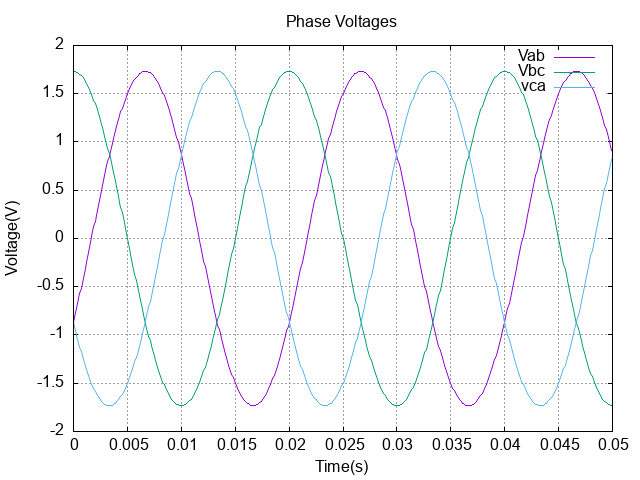
\includegraphics[width=\textwidth]{Phase_Voltages.png}
    \caption{Phase Voltages}
    \label{fig:Phase Voltages}
\end{figure}
\subsection{Why Measure Phase Voltage in the First Place?}

Measuring phase voltage is crucial in three-phase electrical systems for
several reasons. Phase voltages are the voltages measured between a single
phase and the neutral point. These measurements are fundamental because:

\subsection{Need for Conversion from Phase to Line Voltage}

In practical applications, especially in power distribution and motor control,
the line voltage is often more relevant than the phase voltage. Line voltage is
the voltage between any two phases in a three-phase system. Conversion from
phase to line voltage is necessary because:

\subsection{Why Dividing by the Square Root of 3 Does Not Work}

Simply dividing the measured phase voltage by the square root of 3 to obtain
the line voltage does not always yield accurate results due to the following
reasons:

\subsection{The Transform Equation and Its Derivation}